\documentclass[14pt]{extbook}
\usepackage{multicol, enumerate, enumitem, hyperref, color, soul, setspace, parskip, fancyhdr} %General Packages
\usepackage{amssymb, amsthm, amsmath, bbm, latexsym, units, mathtools} %Math Packages
\everymath{\displaystyle} %All math in Display Style
% Packages with additional options
\usepackage[headsep=0.5cm,headheight=12pt, left=1 in,right= 1 in,top= 1 in,bottom= 1 in]{geometry}
\usepackage[usenames,dvipsnames]{xcolor}
\usepackage{dashrule}  % Package to use the command below to create lines between items
\newcommand{\litem}[1]{\item#1\hspace*{-1cm}\rule{\textwidth}{0.4pt}}
\pagestyle{fancy}
\lhead{Progress Quiz 3}
\chead{}
\rhead{Version B}
\lfoot{3148-2249}
\cfoot{}
\rfoot{Spring 2021}
\begin{document}

\begin{enumerate}
\litem{
Solve the radical equation below. Then, choose the interval(s) that the solution(s) belongs to.\[ \sqrt{6 x^2 + 18} - \sqrt{-31 x} = 0 \]\begin{enumerate}[label=\Alph*.]
\item \( x \in [-6.6,-3] \)
\item \( x \in [-3.2,0.3] \)
\item \( x_1 \in [0.2, 1.4] \text{ and } x_2 \in [4.5,6.5] \)
\item \( \text{All solutions lead to invalid or complex values in the equation.} \)
\item \( x_1 \in [-6.6, -3] \text{ and } x_2 \in [-6.67,1.33] \)

\end{enumerate} }
\litem{
What is the domain of the function below?\[ f(x) = \sqrt[4]{-8 x - 3} \]\begin{enumerate}[label=\Alph*.]
\item \( [a, \infty), \text{where } a \in [-5.2, -1.1] \)
\item \( (-\infty, a], \text{where } a \in [-7.67, -1.67] \)
\item \( (-\infty, a], \text{ where } a \in [-1.38, 4.62] \)
\item \( (-\infty, \infty) \)
\item \( [a, \infty), \text{where } a \in [-0.6, 1.6] \)

\end{enumerate} }
\litem{
Choose the graph of the equation below.\[ f(x) = - \sqrt{x + 6} + 7 \]\begin{enumerate}[label=\Alph*.]
\begin{multicols}{2}\item 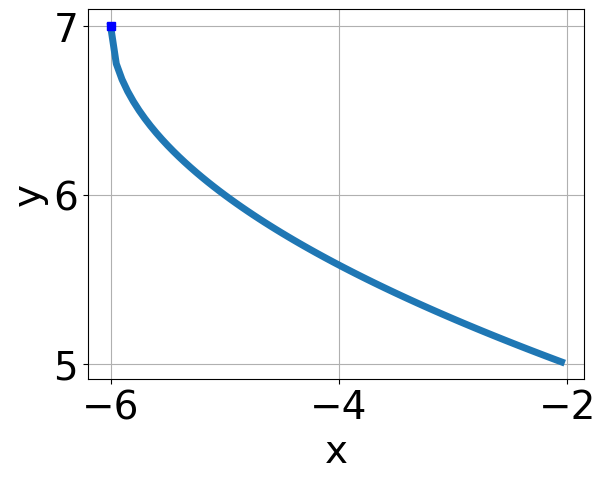
\includegraphics[width = 0.3\textwidth]{../Figures/radicalEquationToGraphAB.png}\item 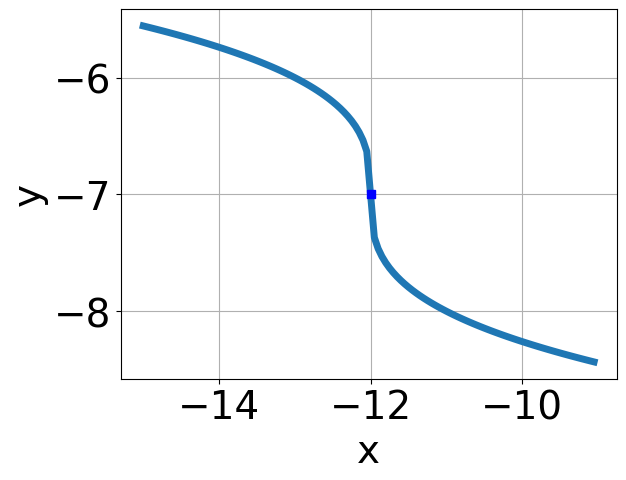
\includegraphics[width = 0.3\textwidth]{../Figures/radicalEquationToGraphBB.png}\item 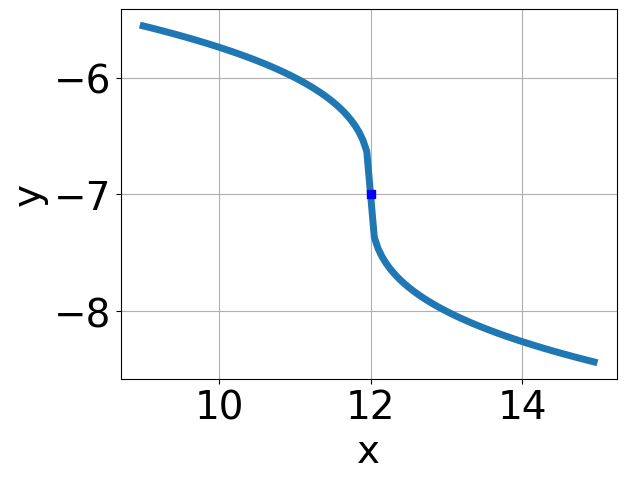
\includegraphics[width = 0.3\textwidth]{../Figures/radicalEquationToGraphCB.png}\item 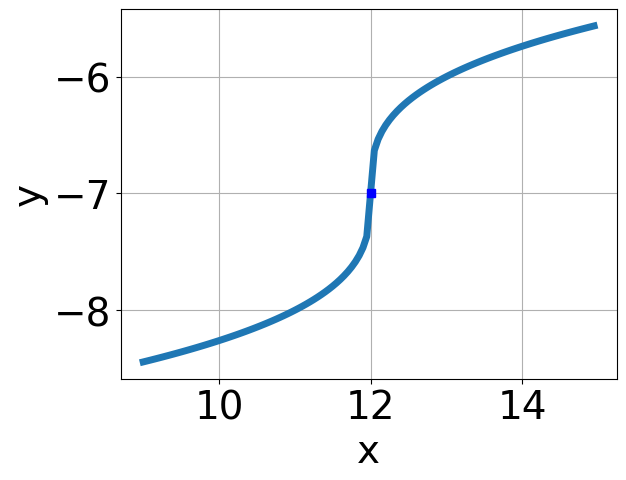
\includegraphics[width = 0.3\textwidth]{../Figures/radicalEquationToGraphDB.png}\end{multicols}\item None of the above.
\end{enumerate} }
\litem{
Choose the graph of the equation below.\[ f(x) = \sqrt{x + 8} - 3 \]\begin{enumerate}[label=\Alph*.]
\begin{multicols}{2}\item 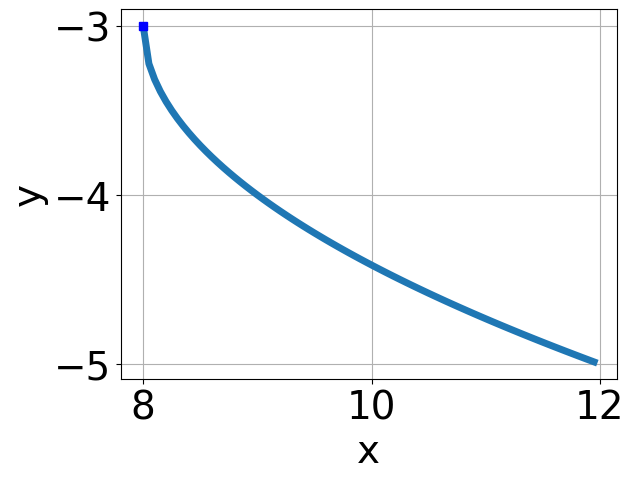
\includegraphics[width = 0.3\textwidth]{../Figures/radicalEquationToGraphCopyAB.png}\item 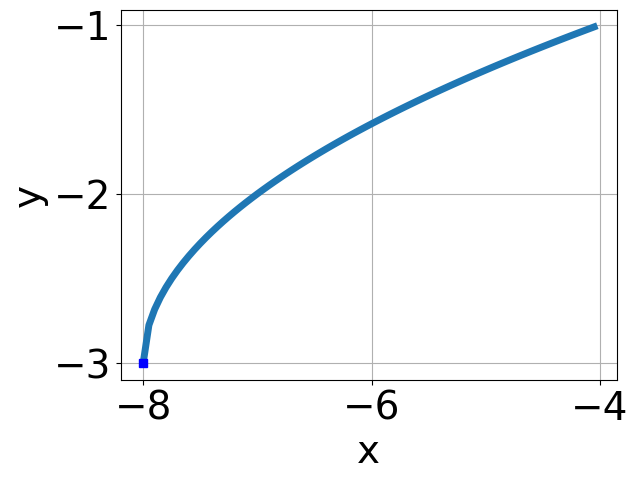
\includegraphics[width = 0.3\textwidth]{../Figures/radicalEquationToGraphCopyBB.png}\item 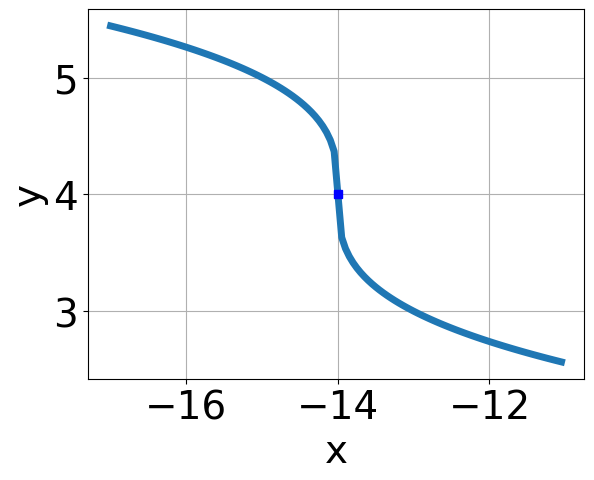
\includegraphics[width = 0.3\textwidth]{../Figures/radicalEquationToGraphCopyCB.png}\item 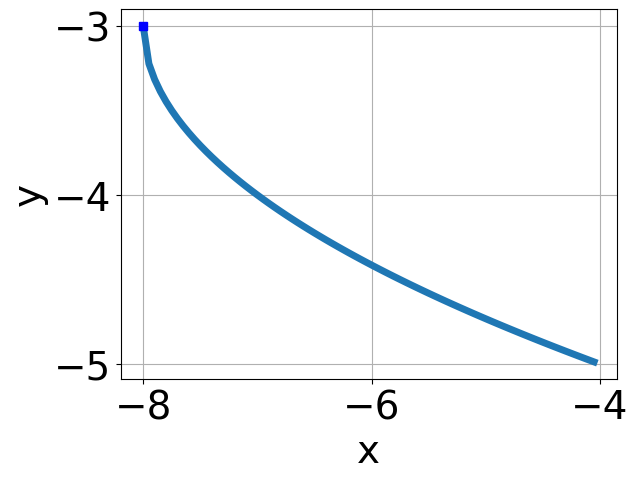
\includegraphics[width = 0.3\textwidth]{../Figures/radicalEquationToGraphCopyDB.png}\end{multicols}\item None of the above.
\end{enumerate} }
\litem{
Solve the radical equation below. Then, choose the interval(s) that the solution(s) belongs to.\[ \sqrt{-32 x^2 + 45} - \sqrt{-4 x} = 0 \]\begin{enumerate}[label=\Alph*.]
\item \( x \in [-1.24,-0.95] \)
\item \( x_1 \in [0.96, 1.17] \text{ and } x_2 \in [0.25,6.25] \)
\item \( x \in [1.15,1.5] \)
\item \( x_1 \in [-1.24, -0.95] \text{ and } x_2 \in [0.25,6.25] \)
\item \( \text{All solutions lead to invalid or complex values in the equation.} \)

\end{enumerate} }
\litem{
Solve the radical equation below. Then, choose the interval(s) that the solution(s) belongs to.\[ \sqrt{-4 x - 3} - \sqrt{-9 x + 7} = 0 \]\begin{enumerate}[label=\Alph*.]
\item \( x_1 \in [-0.76, -0.73] \text{ and } x_2 \in [1.16,2.65] \)
\item \( x \in [2,2.07] \)
\item \( x_1 \in [-0.76, -0.73] \text{ and } x_2 \in [0.67,1.6] \)
\item \( \text{All solutions lead to invalid or complex values in the equation.} \)
\item \( x \in [-0.89,-0.77] \)

\end{enumerate} }
\litem{
What is the domain of the function below?\[ f(x) = \sqrt[8]{-9 x + 5} \]\begin{enumerate}[label=\Alph*.]
\item \( (-\infty, \infty) \)
\item \( [a, \infty), \text{where } a \in [1.7, 3.1] \)
\item \( (-\infty, a], \text{ where } a \in [-1.44, 1.56] \)
\item \( (-\infty, a], \text{where } a \in [0.8, 4.8] \)
\item \( [a, \infty), \text{where } a \in [-2, 0.8] \)

\end{enumerate} }
\litem{
Choose the equation of the function graphed below.
\begin{center}
    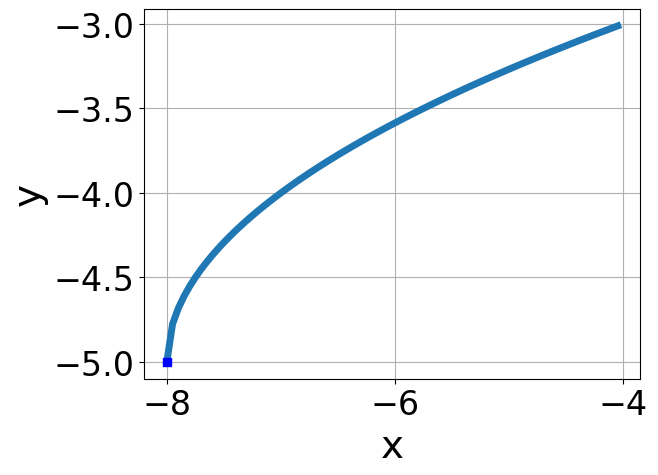
\includegraphics[width=0.5\textwidth]{../Figures/radicalGraphToEquationCopyB.png}
\end{center}
\begin{enumerate}[label=\Alph*.]
\item \( f(x) = \sqrt[3]{x - 12} - 5 \)
\item \( f(x) = \sqrt[3]{x + 12} - 5 \)
\item \( f(x) = - \sqrt[3]{x - 12} - 5 \)
\item \( f(x) = - \sqrt[3]{x + 12} - 5 \)
\item \( \text{None of the above} \)

\end{enumerate} }
\litem{
Choose the equation of the function graphed below.
\begin{center}
    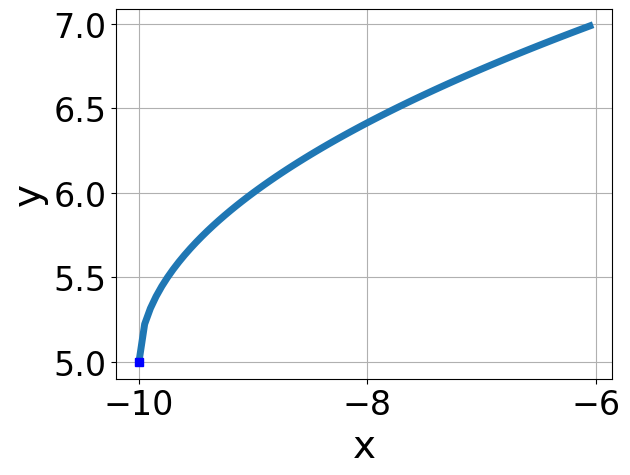
\includegraphics[width=0.5\textwidth]{../Figures/radicalGraphToEquationB.png}
\end{center}
\begin{enumerate}[label=\Alph*.]
\item \( f(x) = \sqrt[3]{x - 10} + 5 \)
\item \( f(x) = - \sqrt[3]{x - 10} + 5 \)
\item \( f(x) = - \sqrt[3]{x + 10} + 5 \)
\item \( f(x) = \sqrt[3]{x + 10} + 5 \)
\item \( \text{None of the above} \)

\end{enumerate} }
\litem{
Solve the radical equation below. Then, choose the interval(s) that the solution(s) belongs to.\[ \sqrt{-3 x - 8} - \sqrt{-9 x - 6} = 0 \]\begin{enumerate}[label=\Alph*.]
\item \( x \in [1.5,4.2] \)
\item \( x_1 \in [-4.2, -0.4] \text{ and } x_2 \in [-0.67,0.33] \)
\item \( \text{All solutions lead to invalid or complex values in the equation.} \)
\item \( x \in [-0.2,1.4] \)
\item \( x_1 \in [-4.2, -0.4] \text{ and } x_2 \in [0.33,1.33] \)

\end{enumerate} }
\end{enumerate}

\end{document}